\subsection{Experimental Setup}
The investigation of unilateral stiffness perturbations on the muscle activation of the contralateral leg was performed using the Variable Stiffness Treadmill (VST) \cite{Barkan_2014_Variable} that has several advantages over other perturbing setups.  These advantages include (1) having a wide range of controllable stiffness while (2) still maintaining high resolution, and (3) it has the ability to actively vary and control the compliance of the treadmill surface within the gait cycle.  The VST is a unique system capable of creating any profile of stiffness during an experiment and throughout the gait cycle.  

\begin{figure}
\centering
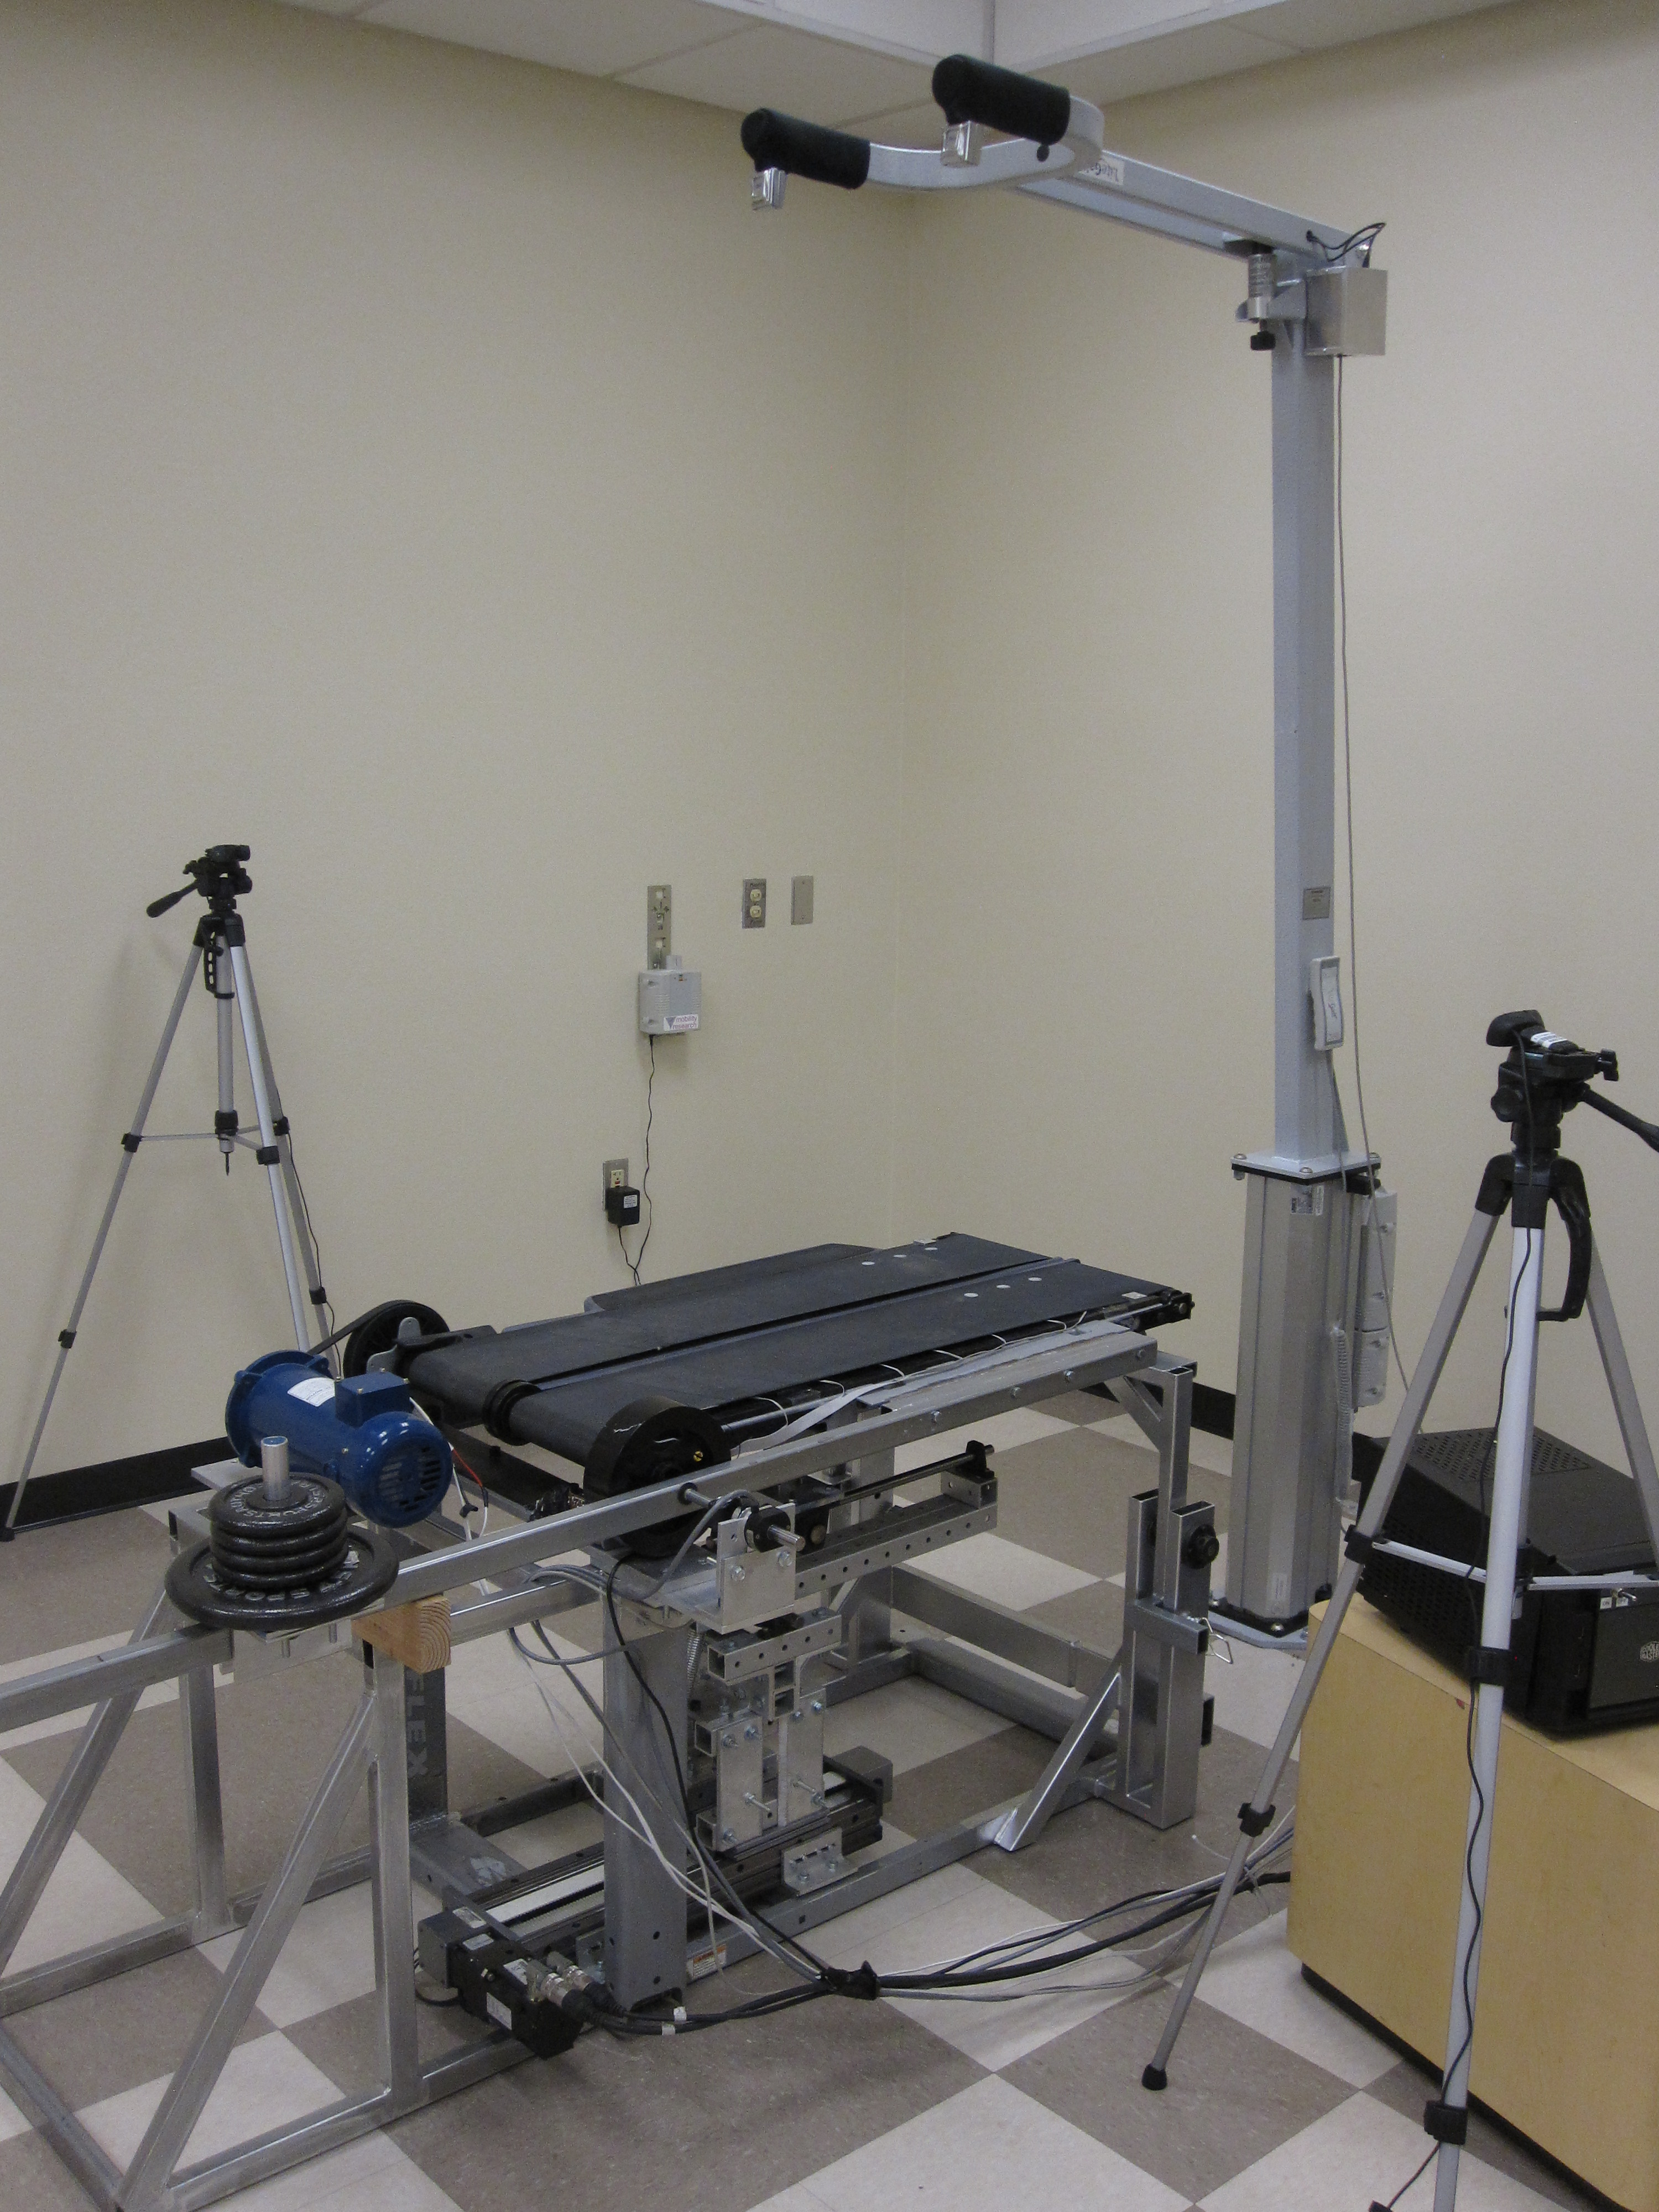
\includegraphics[width=0.7\columnwidth]{Figures/VSTsystem}
\caption{The Variable Stiffness Treadmill system.}
\label{setup}
\end{figure}

%----------------------------------------------------
\subsection{Experimental Protocol}
In order to understand how kinematic feedback of the foot affects inter-limb muscle coordination when body balance is not disturbed we investigated the effect of a stiffness perturbation to one leg on the muscle activity of the contralateral (unperturbed) leg while supplying appox. 30\% body weight support (BWS).  A value of 30\% BWS support has also been employed in other studies that investigated the unilateral effect of length and load sensory feedback on gait \cite{Sinkjaer_2000_Major, AfKlint_2010_Load}.

Four healthy subjects [age 26 SD 5.7 years, weight 190 SD 40 lbs] walked on the treadmill at a speed of $0.70\,m/s$ for over 200 gait cycles.  The right leg was supported by a rigid surface for the duration of this experiment.  The surface under the left leg was commanded to maintain a stiffness of $1\,MN/m$, which is rigid, for 30 gait cycles at the beginning of the experiment.  Then after a random number $i$ of steps, where $i \in \left[ {3,7} \right]$, we immediately dropped the stiffness to 1 of 3 values: $10$, $50$ or $100\,kN/m$.  The low stiffness perturbation began shortly after heel strike and lasted the duration of the left leg stance phase after which the stiffness was commanded back to $1\,MN/m$ for the next $i$ number of steps, as shown in Fig. \ref{show_perturbs}. A minimum of 10 perturbations [15 SD 2.3 perturbations] at each stiffness level were experienced by all subjects.  Informed consent from the subject was obtained at the time of the experiment, and the experimental protocol is approved by the Arizona State University Institutional Review Board (IRB ID\#: STUDY00001001).


NUM healthy subjects [AGE \& WEIGHT DATA] walked on the treadmill at a speed of $0.70\,m/s$ while wearing the virtual reality headset. Two high-framerate infrared cameras (Code Laboratories Inc, model: DUO MINI LX) were used to track the position of infrared emitters (Super Bright LEDs Inc, model: IR-1WS-850) attached to the subject's legs (two markers on each thigh, calf and foot - six per leg, 12 total). The positions of the markers were used to calculate the hip, knee, and ankle joint angles for both legs in real time.

The virtual walking environment was designed with the game development package Unity3D using free gameobjects provided with the software. The virtual world consisted of a cobblestone pathway, fenced in on both sides as shown in RIFT WORLD FIG. Mountains, trees, and tall grass were added for immersive effect. The environment was scaled to realistic sizes, so that walking one meter on the treadmill looked and felt like walking one meter in the virtual world. The speed of the treadmill was automatically synchronised with the movement of the camera view in the environment. In addition, the recorded joint angles were used to control the legs of a virtual avatar. Subjects were given a first-person view of the avatar and, looking down, were able to watch their virtual legs move in time with their actual legs. 

Along the virtual walkway, patches of sand were placed at random intervals on the left side of the path. The locations of these patches were generated randomly each time the experiment was run, adhering to the following two rules: 20 meters of walking before the first sand patch, and 6$\pm$1 meters between each patch, and a total of 120 patches altogether. When the subject's virtual avatar reached a sand patch, one of three types of perturbations would occur. The three types of effected perturbations were the control, the visual-warning-no-stiffness-change, and the no-visual-warning-stiffness-change. The control perturbation was used to train the subject to expect a stiffness change when stepping on the sand patches.

\begin{figure}
\centering
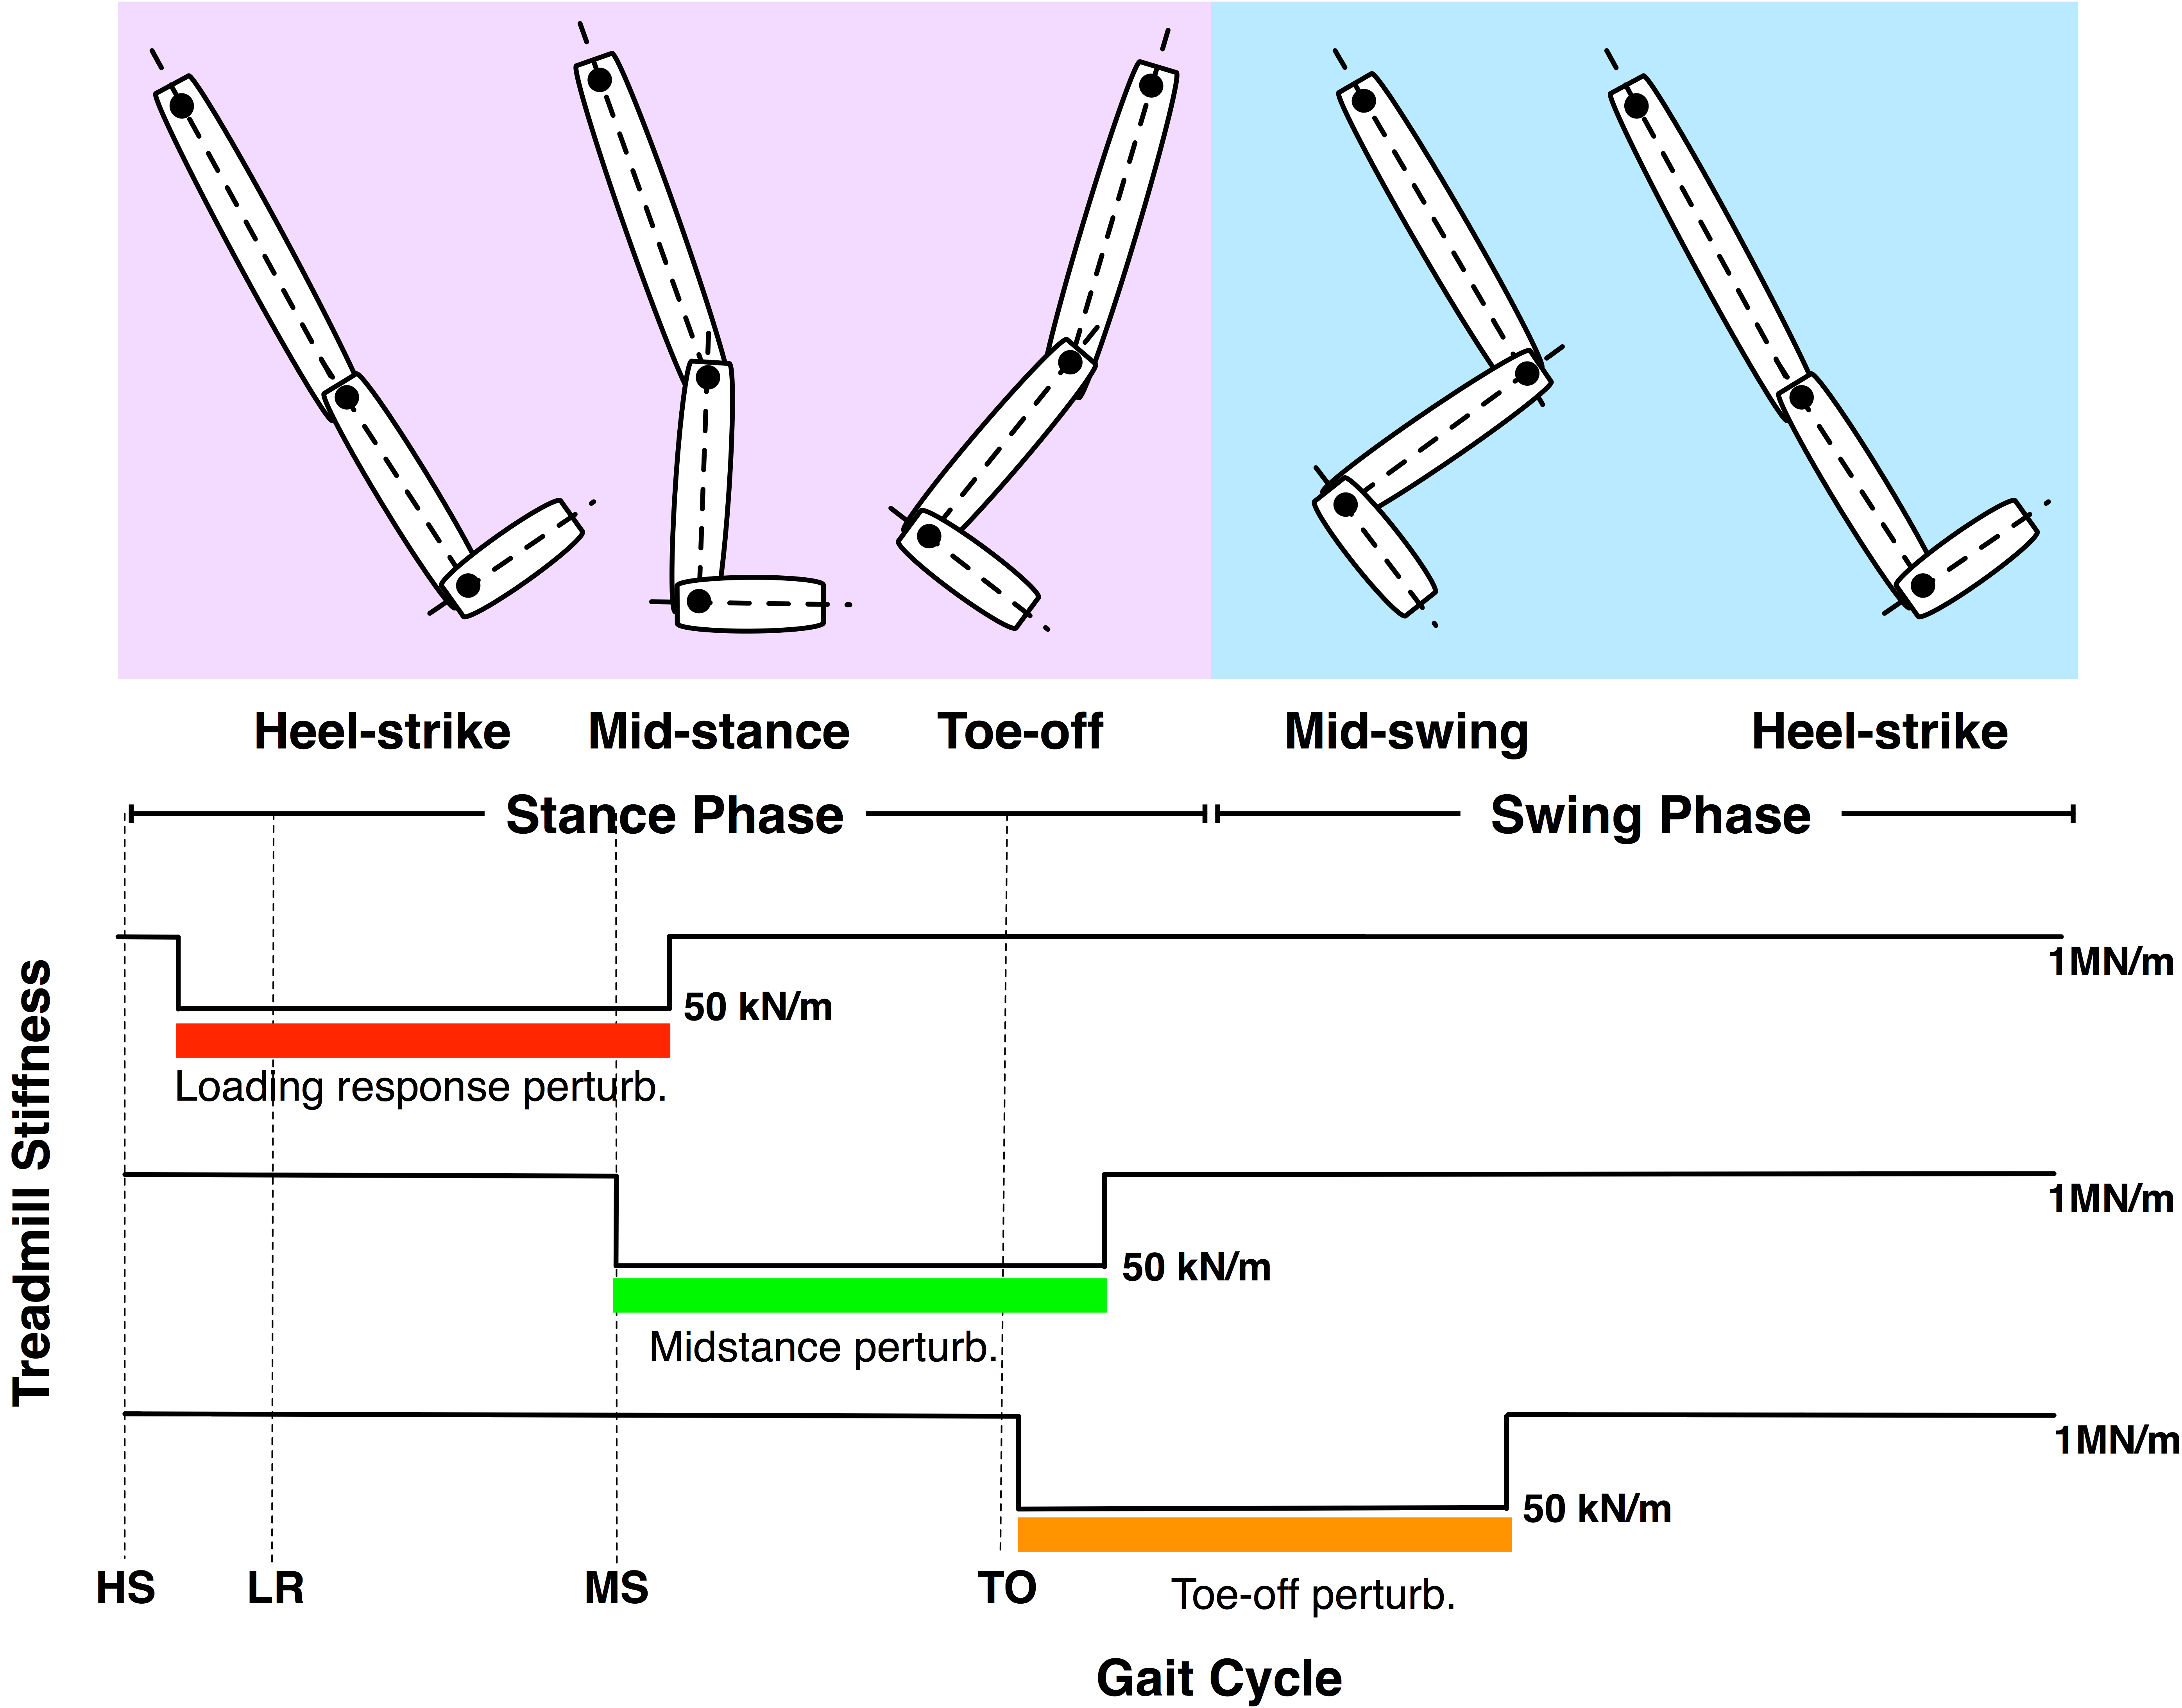
\includegraphics[width=1\columnwidth]{Figures/show_perturbs}
\caption{Timing of unilateral perturbations \J{modify figure}}
\label{show_perturbs}
\end{figure}

The muscle activity of the contralateral leg was obtained by using a wireless surface EMG system (Delsys,  Trigno Wireless EMG) and recorded at $2000$ Hz.  After finding the EMG linear envelope the data was normalized to the maximum value.  Electrodes were placed on the Tibialis Anterior (TA), Gastrocnemous (GA) and Soleous (Sol). The EMG data corresponding to the gait cycles of walking on the rigid surface and the cycles pertaining to the three perturbations was found and normalized temporally to percent gait cycle to eliminate discrepancies due to natural variations in gait patterns (i.e. stride length, cycle time, etc).  The first 30 gait cycles and the cycles in between perturbations at infinite stiffness (except for two cycles following a perturbation to eliminate any residual effects from the perturbation) are included in the unperturbed (i.e. ``rigid'') data set.  This results in normalized EMG as a function of percent gait cycle, where 0\% corresponds to the heel strike of the left leg.

% Add this in
%Kinematic data for both legs was obtained using a motion capture system (Code Laboratories Inc, model: DUO MINI LX) that was used to track 12 infrared LEDs (Super Bright LEDs Inc, model: IR-1WS-850) placed on the thigh, shank, and foot as shown in Fig. \J{Insert pic} in order to calculate the joint angles throughout the gait cycle. 





